\chapter{Рассеяние, дуальность и амплитуда Венециано}

\lectureoverview{Рассеяние сводит столкновение к инвариантным данным, которые можно сопоставить с экспериментом. Для четырёх одинаковых частиц эти данные можно организовать в переменные Мандельстама \(s,t,u\), из которых независимы только две. Тогда обычная картина обмена частицами подсказывает отдельные прямой и перекрёстный каналы. Амплитуда Венециано опровергла это ожидание: одна функция содержит описание обоих каналов. Во второй половине лекции эта функция строится из двух открытых струн, которые соединяются, эволюционируют как одна колеблющаяся цепь и затем вновь расщепляются.}

\section{Что должна предсказывать теория}

Фермионные струны устраняют два дефекта чисто бозонной модели: они допускают фермионные состояния и, после соответствующей проекции, устраняют тахион. Их критическая размерность пространства-времени равна десяти, а не двадцати шести. Следовательно, дополнительные измерения по-прежнему остаются, но их компактификация пока откладывается. Непосредственная тема — рассеяние.
\editorialnote{Утверждение об отсутствии тахиона относится к согласованному спектру суперструны после необходимой проекции; простого добавления фермионов мирового листа само по себе недостаточно.}

Рассеяние не обязательно самое интересное из того, что могут делать частицы. Это просто тот процесс, который в эксперименте можно чисто воспроизводить. Направьте заданные частицы навстречу друг другу, зарегистрируйте частицы, выходящие из столкновения, и сделайте вывод о динамике, скрытой внутри области взаимодействия. Теория становится количественной, когда задаёт комплексную амплитуду
\begin{equation}
  \mathcal A(\hbox{incoming data}\to\hbox{outgoing data}),
\end{equation}
квадрат модуля которой вместе с обычными фазово-пространственными факторами даёт вероятность такого исхода.

\begin{figure}[H]
  \centering
  
\includegraphics[width=0.72\textwidth]{lecture_06_figure_01.png}
  \caption{Входящие частицы входят в область взаимодействия, изображённую как чёрный ящик, а выходящие появляются из неё; время отложено по горизонтали.}
  \lectureframe{00:02:35}
  \label{fig:l06-black-box}
\end{figure}

Частицы также несут спин, заряд и метки типа. Чтобы сначала выделить кинематику, временно опустим всё, кроме импульса.

\section{Четырёхимпульс и соглашение о всех входящих импульсах}

Запишем четырёхимпульс одной частицы в виде
\begin{equation}
  k^\mu=(k^0,\mathbf k)=(E,\mathbf p).
\end{equation}
В лекции используется метрика с преимущественно положительной сигнатурой, поэтому
\begin{equation}
  k^2\equiv \mathbf p^2-E^2.
\end{equation}
Следовательно, релятивистское дисперсионное соотношение имеет вид
\begin{equation}
  E^2-\mathbf p^2=m^2,
  \qquad
  k^2=-m^2.
  \label{eq:l06-mass-shell}
\end{equation}
Изменение пространственного импульса меняет энергию, но не уводит частицу с её массовой поверхности.

\begin{figure}[H]
  \centering
  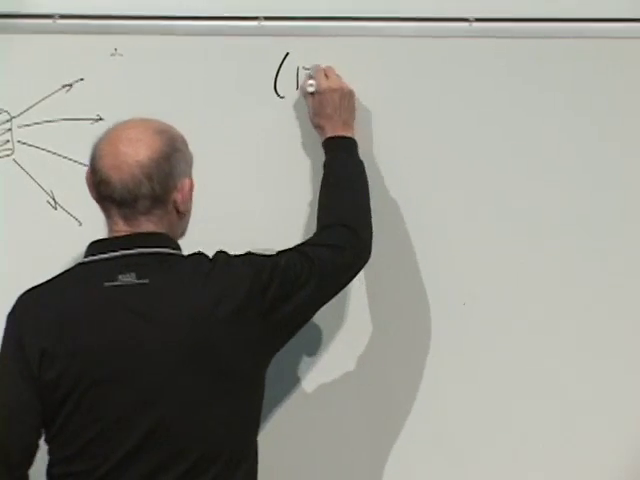
\includegraphics[width=0.66\textwidth]{lecture_06_figure_02.png}
  \caption{Условие массовой поверхности в метрической конвенции, используемой на протяжении всей лекции.}
  \lectureframe{00:05:56}
  \label{fig:l06-mass-shell}
\end{figure}

Рассмотрим две входящие частицы с импульсами \(k_1,k_2\) и две выходящие с физическими импульсами \(q_3,q_4\). Сохранение энергии и импульса выражается одним уравнением для четырёхвектора,
\begin{equation}
  k_1+k_2=q_3+q_4.
  \label{eq:l06-physical-conservation}
\end{equation}
Удобно приписать каждой внешней линии входящий импульс:
\begin{equation}
  k_3\equiv-q_3,
  \qquad
  k_4\equiv-q_4.
\end{equation}
Тогда
\begin{equation}
  k_1+k_2+k_3+k_4=0,
  \label{eq:l06-all-incoming}
\end{equation}
и каждая внешняя линия подчиняется условию \(k_i^2=-m_i^2\). У выходящих частиц отрицательная энергия возникает только в этой условной записи; их физические энергии остаются положительными.

\begin{figure}[H]
  \centering
  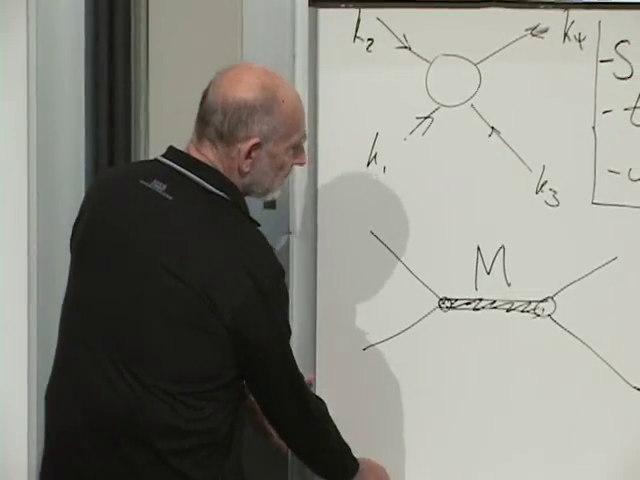
\includegraphics[width=0.68\textwidth]{lecture_06_figure_03.png}
  \caption{Физические выходящие импульсы меняют знак, чтобы все четыре внешних импульса можно было симметрично рассматривать как входящие.}
  \lectureframe{00:09:10}
  \label{fig:l06-all-incoming-board}
\end{figure}

На первый взгляд амплитуда кажется функцией шестнадцати компонент, \(\mathcal A(k_1,k_2,k_3,k_4)\). Большинство из них избыточны. Перейдём в систему центра масс, повернём входящие импульсы вдоль выбранной оси и для простоты предположим, что все четыре частицы имеют одинаковую массу. Тогда входящее состояние задаётся одним числом — энергией в системе центра масс. Пространственные импульсы на выходе должны быть равны по модулю и противоположны по направлению и иметь тот же модуль, что и у входящей пары. Остаётся только угол их отклонения \(\theta\). Следовательно, процесс имеет две независимые кинематические переменные:
\begin{equation}
  E_{\mathrm{cm}},
  \qquad
  \theta.
  \label{eq:l06-two-data}
\end{equation}

\section{Переменные Мандельстама}

Две физические величины в \eqref{eq:l06-two-data} должны выражаться без выбора системы отсчёта. При соглашении, в котором все импульсы считаются входящими, определим
\begin{equation}
  \begin{aligned}
    -s&=(k_1+k_2)^2,\\
    -t&=(k_1+k_3)^2,\\
    -u&=(k_1+k_4)^2.
  \end{aligned}
  \label{eq:l06-mandelstam}
\end{equation}
В системе центра масс пространственные части \(k_1+k_2\) сокращаются, поэтому
\begin{equation}
  s=E_{\mathrm{cm}}^2.
  \label{eq:l06-s-energy}
\end{equation}

Для физического выходящего импульса \(q_3=-k_3\)
\begin{equation}
  k_1+k_3=k_1-q_3
\end{equation}
представляет собой импульс, переданный от линии 1 к линии 3. При равных внешних массах и модуле входящего пространственного импульса \(p\)
\begin{equation}
  -t=2p^2(1-\cos\theta),
  \qquad
  -u=2p^2(1+\cos\theta).
  \label{eq:l06-tu-angle}
\end{equation}
Следовательно, \(t\) и \(u\) несут угловую информацию, измеряемую детекторами.

\begin{figure}[H]
  \centering
  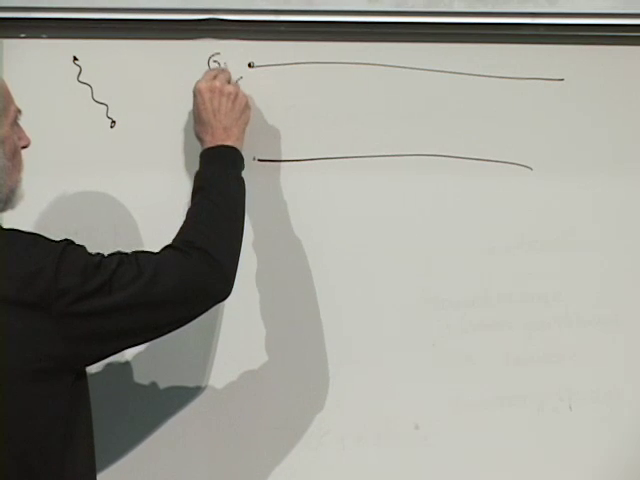
\includegraphics[width=0.74\textwidth]{lecture_06_figure_04.png}
  \caption{Симметричные определения \(s,t,u\) при соглашении о всех входящих импульсах.}
  \lectureframe{00:26:20}
  \label{fig:l06-stu-board}
\end{figure}

Три символа не означают трёх независимых величин. Возведя \eqref{eq:l06-all-incoming} в квадрат и используя \(k_i^2=-m^2\), получаем
\begin{equation}
  s+t+u=4m^2
  \label{eq:l06-stu-constraint}
\end{equation}
для равных масс. Как только известны \(s\) и \(t\), \(u\) фиксируется.

\begin{classroomqa}
\audiencequestion{Может ли вакуум замедлять свободно движущуюся частицу, подобно трению? \lecturetimestamp{00:27:17}}
\lecturerresponse{Не в вакууме, инвариантном относительно трансляций. Недостающему импульсу некуда деться, так что сохранение импульса запрещает такое трение. Можно вообразить среду или другой вакуум, который выделяет предпочтительную систему покоя, но здесь используется не такой вакуум.}
\end{classroomqa}

\begin{classroomqa}
\audiencequestion{Почему две выходящие частицы должны иметь одинаковые энергии? \lecturetimestamp{00:27:54}}
\lecturerresponse{В системе центра масс их пространственные импульсы должны быть равны по модулю и противоположны по направлению. Для обсуждаемого процесса с равными массами равенство модулей импульсов влечёт равенство энергий через
\(E^2=p^2+m^2\). Если бы массы выходящих частиц различались, этот последний вывод пришлось бы изменить.}
\end{classroomqa}

\section{Прямой и перекрёстный каналы}

Простая диаграмма точечных частиц позволяет частицам 1 и 2 образовать промежуточную частицу массы \(M\), которая затем распадается на 3 и 4. С точностью до множителей в числителе и предписания обхода полюса характерная зависимость имеет вид
\begin{equation}
  \mathcal A_s\sim\frac{g^2}{s-M^2}.
  \label{eq:l06-s-channel}
\end{equation}
Это прямой, или процесс в \(s\)-канале. Если повернуть схему соединения набок, получится обмен между двумя внешними линиями,
\begin{equation}
  \mathcal A_t\sim\frac{g^2}{t-M^2},
  \label{eq:l06-t-channel}
\end{equation}
— перекрёстный, или процесс в \(t\)-канале. Третья схема соединения даёт
\begin{equation}
  \mathcal A_u\sim\frac{g^2}{u-M^2}.
  \label{eq:l06-u-channel}
\end{equation}

\begin{figure}[H]
  \centering
  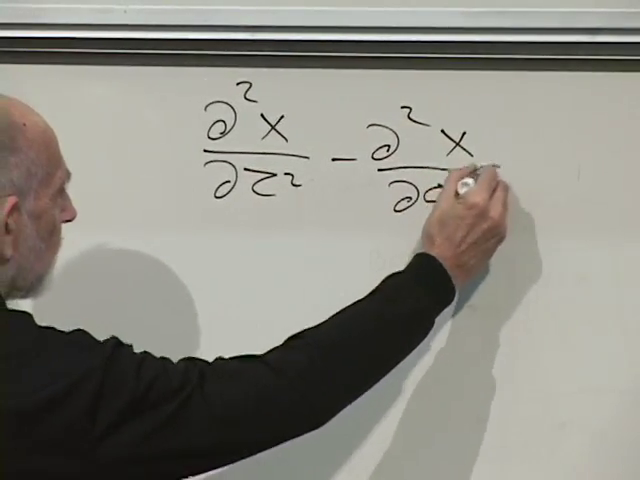
\includegraphics[width=0.72\textwidth]{lecture_06_figure_05.png}
  \caption{Прямое образование через промежуточное состояние и соответствующий полюс \(g^2/(s-M^2)\); на той же доске собирается перекрёстная схема соединения.}
  \lectureframe{00:30:50}
  \label{fig:l06-channel-board}
\end{figure}

Различие здесь физическое. На этом грубом скалярном уровне \eqref{eq:l06-s-channel} зависит от энергии столкновения, но не от угла. Составное состояние успевает забыть первоначальное направление до распада, поэтому его распад изотропен. Амплитуда обмена зависит от переданного импульса и, следовательно, от угла; лёгкая обмениваемая частица резко предпочитает малое отклонение. Спин добавил бы дополнительную угловую зависимость, но полюсная структура уже видна.

\begin{classroomqa}
\audiencequestion{Даёт ли отсутствующий \(u\)-канал третий член? \lecturetimestamp{00:34:47}}
\lecturerresponse{Да, всякий раз, когда типы частиц и константы связи допускают такую схему соединения. Тогда включают член с полюсом при \(u=M^2\). Это не новая независимая кинематическая переменная, поскольку
\(s+t+u=4m^2\), но это отдельная диаграмма канала.}
\end{classroomqa}

\section{Одна функция, два описания каналов}

Один полюс — плохая модель рассеяния мезонов. Два мезона могут образовать много резонансов, с целой башней масс и угловых моментов. Первой реакцией в 1960-е годы было добавить больше полюсов \(s\)-канала, больше полюсов \(t\)-канала и разрешённые полюса \(u\)-канала. Затем была найдена гораздо более экономичная функция. В единицах, используемых в лекции, где линейная траектория Редже и её интерсепт поглощены в \(s\) и \(t\), она имеет вид
\begin{equation}
  \mathcal A_{\mathrm V}(s,t)
  \propto
  \frac{\Gamma(-s)\Gamma(-t)}{\Gamma(-s-t)}.
  \label{eq:l06-veneziano}
\end{equation}
Гамма-функция продолжает факториал:
\begin{equation}
  \Gamma(n)=(n-1)!
\end{equation}
при положительных целых значениях.

\begin{figure}[H]
  \centering
  \includegraphics[width=0.68\textwidth]{lecture_06_figure_06.png}
  \caption{Амплитуда Венециано, записанная как симметричное отношение гамма-функций.}
  \lectureframe{00:42:25}
  \label{fig:l06-veneziano-board}
\end{figure}

Полюса \(\Gamma(-s)\) воспроизводят бесконечную башню резонансов прямого канала. Однако то же выражение симметрично относительно \(s\leftrightarrow
t\), так что его полюса \(\Gamma(-t)\) дают разложение по перекрёстному каналу. Это не два вклада, добавленные по отдельности. Одна аналитическая функция допускает любое из двух описаний. Это старая идея дуальности между резонансами прямого канала и обменами в перекрёстном канале.

\begin{classroomqa}
\audiencequestion{Как одна амплитуда может содержать суммы по обоим каналам без их сложения? \lecturetimestamp{00:43:32}}
\lecturerresponse{В этом-то и состоит неожиданность. Разложение функции вблизи её полюсов \(s\)-канала даёт описание в терминах прямых резонансов; разложение той же функции вблизи её полюсов \(t\)-канала даёт описание в терминах обменов. Чтобы объяснить, почему эти два прочтения совпадают, нужна микроскопическая модель, и этой моделью является взаимодействующая струна.}
\end{classroomqa}

\section{Полоса, заметаемая открытой струной}

Параметризуем открытую струну так:
\begin{equation}
  0\leq\sigma\leq\pi.
\end{equation}
Метка \(\sigma\) не является координатой пространства-времени. Вложение
\(X^\mu(\sigma,\tau)\) указывает, где в пространстве-времени находится точка с этой меткой,
тогда как \(\tau\) измеряет эволюцию. Точечная частица заметает мировую линию;
движущаяся струна заметает двумерный мировой лист. В свободной
теории каждая координата вложения удовлетворяет
\begin{equation}
  \frac{\partial^2X^\mu}{\partial\tau^2}
  -
  \frac{\partial^2X^\mu}{\partial\sigma^2}
  =0.
  \label{eq:l06-wave-equation}
\end{equation}

\begin{figure}[H]
  \centering
  \includegraphics[width=0.70\textwidth]{lecture_06_figure_07.png}
  \caption{Волновое уравнение, которому подчиняется каждая координата свободной струны на полосе мирового листа.}
  \lectureframe{00:49:10}
  \label{fig:l06-wave-equation-board}
\end{figure}

Для построения рассеяния полезно не переходить к пределу континуума слишком рано. Заменим каждую струну \(n\) материальными точками, соединёнными пружинами.
Мировой лист превращается в плотное множество близких мировых линий, а его
нормальные моды — в обычные гармонические осцилляторы. Две входящие цепочки могут
соприкоснуться своими концами. В этот момент новая пружина соединяет их, они
эволюционируют в течение времени \(\tau\) как одна более длинная цепочка, а позже
одна пружина разрывается, так что возникают две выходящие цепочки.

\begin{figure}[H]
  \centering
  \includegraphics[width=0.72\textwidth]{lecture_06_figure_08.png}
  \medskip

  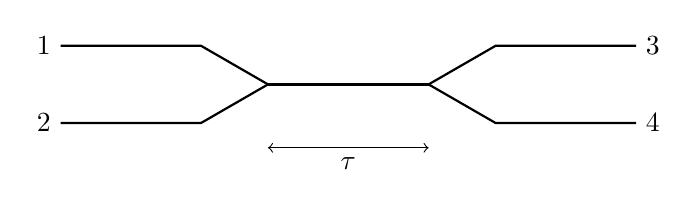
\begin{tikzpicture}[x=0.85cm,y=0.70cm]
    \draw[thick] (0,2.2) -- (2.1,2.2) -- (3.1,1.5);
    \draw[thick] (0,0.8) -- (2.1,0.8) -- (3.1,1.5);
    \draw[thick] (3.1,1.5) -- (5.5,1.5);
    \draw[thick] (5.5,1.5) -- (6.5,2.2) -- (8.6,2.2);
    \draw[thick] (5.5,1.5) -- (6.5,0.8) -- (8.6,0.8);
    \draw[<->] (3.1,0.35) -- node[below] {\(\tau\)} (5.5,0.35);
    \node[left] at (0,2.2) {1};
    \node[left] at (0,0.8) {2};
    \node[right] at (8.6,2.2) {3};
    \node[right] at (8.6,0.8) {4};
  \end{tikzpicture}
  \caption{Две дискретизованные открытые струны соприкасаются, образуют одну промежуточную струну
  на время \(\tau\), а затем расщепляются. Исходный кадр сохраняет
  конструкцию из пружин и мировых линий; схема выделяет только её
  связность.}
  \lectureframe{00:51:25}
  \label{fig:l06-string-joining}
\end{figure}

Две струны изображены рядом лишь в пространстве параметров. Их положения в пространстве-времени
не обязаны быть соседними, пока координаты концов действительно не
совпадут. Свобода перепараметризации позволяет помещать события
соединения и расщепления в удобные места на диаграмме; на следующей лекции эта геометрическая свобода
станет конформной симметрией.

\section{Осцилляторное вычисление в замедленном темпе}

Пусть у первой цепочки координаты \(x_1,\ldots,x_n\), а у второй
\(x_{n+1},\ldots,x_{2n}\). Их координаты центра масс таковы:
\begin{equation}
  X_{\mathrm{cm}}^{(1)}
  =\frac1n\sum_{a=1}^{n}x_a,
  \qquad
  X_{\mathrm{cm}}^{(2)}
  =\frac1n\sum_{a=n+1}^{2n}x_a.
  \label{eq:l06-chain-centers}
\end{equation}
Цепочка с определённым импульсом \(k_1\) имеет плоскую волну центра масс,
умноженную на внутреннее основное осцилляторное состояние:
\begin{align}
  \Psi_1
  &=
  e^{ik_1\cdot X_{\mathrm{cm}}^{(1)}}
  \psi_0(x_1,\ldots,x_n),
  \\
  \Psi_2
  &=
  e^{ik_2\cdot X_{\mathrm{cm}}^{(2)}}
  \psi_0(x_{n+1},\ldots,x_{2n}).
  \label{eq:l06-two-wavefunctions}
\end{align}
Множители \(\psi_0\) зависят от относительных координат, а не от общего
переноса всей цепочки. Поскольку входящие струны изначально являются
отдельными квантовыми системами,
\begin{equation}
  \Psi_{\mathrm{in}}=\Psi_1\Psi_2.
  \label{eq:l06-product-state}
\end{equation}

\begin{figure}[H]
  \centering
  \includegraphics[width=0.76\textwidth]{lecture_06_figure_09.png}
  \caption{Две импульсные плоские волны и множители их внутренних основных осцилляторных
  состояний, записанные разными цветами.}
  \lectureframe{00:58:05}
  \label{fig:l06-wavefunctions-board}
\end{figure}

Соединение выделяет ту часть этой волновой функции, для которой совпадают
две координаты концов:
\begin{equation}
  x_n=x_{n+1}.
  \label{eq:l06-endpoint-contact}
\end{equation}
В этот момент остальные координаты не изменяются. Затем выделенное состояние
эволюционирует с гамильтонианом \(H_{\mathrm{joined}}\) одной
более длинной цепочки:
\begin{equation}
  \Psi(\tau)
  =
  e^{-iH_{\mathrm{joined}}\tau}\Psi(0).
  \label{eq:l06-time-evolution}
\end{equation}
Наконец, берут его перекрытие с произведением состояний выходящих струн,
несущих импульсы \(q_3,q_4\).

\begin{figure}[H]
  \centering
  \includegraphics[width=0.76\textwidth]{lecture_06_figure_10.png}
  \caption{Волновая функция двух цепочек непосредственно перед тем,
  как налагается условие совпадения концов.}
  \lectureframe{00:58:55}
  \label{fig:l06-endpoint-board}
\end{figure}

Вычисление длинное, но не загадочное. Каждую внутреннюю координату
можно разложить по осцилляторным модам, так что перекрытие при соединении, временная
эволюция и конечная проекция сводятся к гауссовой алгебре осцилляторов.
Неопределённым остаётся время жизни \(\tau\) соединённой струны.

\begin{classroomqa}
\audiencequestion{Чёрная и красная волновые функции складываются или
перемножаются? \lecturetimestamp{01:02:26}}
\lecturerresponse{Перемножаются. Состояние, являющееся тензорным произведением двух независимых
систем, в координатном базисе представляется произведением их
волновых функций. Сложение описывало бы суперпозицию альтернатив, а не
одновременное присутствие обеих входящих струн.}
\end{classroomqa}

\begin{classroomqa}
\audiencequestion{Почему нужно интегрировать по промежуточному времени
\(\tau\)? \lecturetimestamp{01:04:04}}
\lecturerresponse{Соединённой струне не приписывается фиксированное время жизни.
Правило Фейнмана состоит в том, чтобы суммировать амплитуды по всем допустимым историям. В этом
описании оставшимся непрерывным параметром истории является время между
соединением и расщеплением, поэтому сумма превращается в интеграл по
\(0\leq\tau<\infty\).}
\end{classroomqa}

\section{От времени распространения к бета-функции}

После вычисления перекрытий осцилляторных состояний результат можно записать в виде
\begin{equation}
  \mathcal A(s,t)
  \propto
  \int_0^\infty d\tau\,
  e^{\tau(s+1)}
  \bigl(1-e^{-\tau}\bigr)^{-t-1}
  e^{-\tau}.
  \label{eq:l06-tau-integral}
\end{equation}
Последний множитель \(e^{-\tau}\) оставлен явно, поскольку именно он даёт якобиан,
необходимый на следующем шаге. Эквивалентно, первая и последняя экспоненты объединяются в
\(e^{s\tau}\).

\begin{figure}[H]
  \centering
  \includegraphics[width=0.76\textwidth]{lecture_06_figure_11.png}
  \caption{Подынтегральное выражение по времени распространения после осцилляторного вычисления;
  отдельный множитель \(e^{-\tau}\) даёт якобиан при замене
  переменной.}
  \lectureframe{01:06:45}
  \label{fig:l06-tau-integral-board}
\end{figure}

Теперь положим
\begin{equation}
  z=e^{-\tau},
  \qquad
  dz=-e^{-\tau}\,d\tau.
  \label{eq:l06-z-substitution}
\end{equation}
Когда \(\tau\) изменяется от \(0\) до \(\infty\), \(z\) изменяется от \(1\) до \(0\).
Знак минус меняет пределы местами, и получается
\begin{equation}
  \mathcal A(s,t)
  \propto
  \int_0^1
  z^{-s-1}(1-z)^{-t-1}\,dz.
  \label{eq:l06-beta-integral}
\end{equation}

\begin{figure}[H]
  \centering
  \includegraphics[width=0.74\textwidth]{lecture_06_figure_12.png}
  \caption{Подстановка \(z=e^{-\tau}\) делает явным эйлеров интеграл
  для бета-функции.}
  \lectureframe{01:08:49}
  \label{fig:l06-beta-integral-board}
\end{figure}

Этот интеграл непосредственно определён там, где он сходится на пределах интегрирования, а
в остальных случаях — аналитическим продолжением. Это бета-функция Эйлера:
\begin{equation}
  B(-s,-t)
  =
  \frac{\Gamma(-s)\Gamma(-t)}{\Gamma(-s-t)}.
  \label{eq:l06-beta-gamma}
\end{equation}

\begin{figure}[H]
  \centering
  \includegraphics[width=0.72\textwidth]{lecture_06_figure_13.png}
  \caption{На доске преобразованный интеграл отождествляется с
  \(B(-s,-t)\) и начинается восстановление его формы через гамма-функции.}
  \lectureframe{01:12:24}
  \label{fig:l06-beta-gamma-board}
\end{figure}

Симметрия по каналам теперь элементарна. При \(z\mapsto1-z\),
\begin{equation}
  \int_0^1 z^{-s-1}(1-z)^{-t-1}\,dz
  =
  \int_0^1 z^{-t-1}(1-z)^{-s-1}\,dz.
\end{equation}
Следовательно, \(\mathcal A(s,t)=\mathcal A(t,s)\). Процесс, построенный как соединение двух
струн с последующим расщеплением, автоматически включает и перекрёстное
описание.
\editorialnote{На лекции в аргументах бета-функции опущены наклон траектории Редже и интерсепт. В стандартных обозначениях \(s,t\) заменяют
соответствующими линейными траекториями \(\alpha(s),\alpha(t)\). Дуальность и довод с заменой переменной при этом не меняются.}

\begin{classroomqa}
\audiencequestion{Отношение гамма-функций похоже на факториальные выражения
в комбинаторике. Есть ли у этого прямое физическое
истолкование как подсчёта? \lecturetimestamp{01:13:22}}
\lecturerresponse{При целых аргументах бета-функция связана с
отношением вроде \(n!\,m!/(n+m)!\), но здесь не утверждается никакого
комбинаторного механизма. Та же специальная функция просто возникает из
интеграла по мировому листу; это сходство не было тем путём, которым была найдена
амплитуда.}
\end{classroomqa}

Пока ещё скрытая причина того, что один мировой лист можно интерпретировать в обоих каналах, — это
конформная симметрия. Она позволяет растягивать лист словно тянучку, не
изменяя амплитуды, превращая длинную область распространения в прямом канале
в картину обмена в перекрёстном канале. Это геометрическое объяснение
отложено до следующей лекции.

\section{Что установила проверка на рассеянии}
\enlargethispage{3\baselineskip}
\begingroup
\setlength{\medskipamount}{3pt plus 1pt minus 1pt}

Дискретная картина соединения вызвала последнюю серию вопросов.

\begin{classroomqa}
\audiencequestion{Если две цепочки из \(n\) составляющих соединяются своими
концами, получается ли \(2n-1\), и может ли это изменить фермионную
чётность? \lecturetimestamp{01:16:16}}
\lecturerresponse{В адронной картине концов соприкасающуюся пару
концов можно рассматривать как пару частица-античастица, которая аннигилирует, так
что число уменьшается на два, а не на один. В пределе континуума конечная
разность между \(2n\) и \(2n-2\) несущественна, а вот сохранение фермионной
чётности — нет. Решёточные составляющие служат лишь регуляризацией непрерывной
струны, а не буквальными фундаментальными бусинами.}
\end{classroomqa}

\begin{classroomqa}
\audiencequestion{Продолжится ли дальнейшее обсуждение вплоть до полной
математики суперструн? \lecturetimestamp{01:18:05}}
\lecturerresponse{Будут использоваться только отдельные следствия. Непосредственный
путь идёт через симметрию мирового листа и компактификацию, а затем — через
иную отправную точку, разработанную в середине 1990-х годов: М-теорию. Её назначение
состоит в том, чтобы прийти к той же физике с точки зрения, в которой несколько
иначе сложных черт становятся прозрачными.}
\end{classroomqa}

\begin{classroomqa}
\audiencequestion{Было ли это правило соединения лишь подсказкой,
пришедшей из столкновений мезонов? \lecturetimestamp{01:20:02}}
\lecturerresponse{Рассеяние мезонов дало историческую подсказку, но это
правило является общим для открытых струн. Та же топология описывает столкновения
открыто-струнных фотонов и других состояний открытой струны. Две замкнутые струны
соединяются и расщепляются аналогичным образом, причём в
промежуточной области находится замкнутая струна.}
\end{classroomqa}

\begin{classroomqa}
\audiencequestion{Применимо ли это вычисление только тогда, когда состояния струны являются
фермионами? \lecturetimestamp{01:20:56}}
\lecturerresponse{Нет. Исходное вычисление Венециано относится к
бозонной открытой струне. Суперструны требуют дополнительных фермионных степеней
свободы и меняют детали подынтегрального выражения, но логика соединения, распространения,
проекции и дуальности мирового листа остаётся в близкой степени аналогичной.}
\end{classroomqa}

Обнаружение в осцилляторном спектре состояния со спином 1 или 2 было наводящим на мысль, но не решающим. Их амплитуды рассеяния послужили более сильной проверкой. Фотонные амплитуды удовлетворяют тождествам, связанным с сохранением заряда и калибровочной инвариантностью; амплитуды гравитона удовлетворяют соответствующим ограничениям безмассового поля со спином 2. Эти струнные состояния выдержали эти проверки во взаимодействиях с массивными и безмассовыми состояниями и друг с другом. Именно поэтому обозначения «фотон» и «гравитон» стали физическими отождествлениями, а не догадками, основанными только на подсчёте поляризаций.
\editorialnote{В современной терминологии эти проверки закодированы в расцеплении нефизических поляризаций, калибровочных тождествах Уорда и универсальном низкоэнергетическом взаимодействии безмассового состояния со спином 2.}

\begin{classroomqa}
\audiencequestion{Откуда в струнном описании берётся сам электрический заряд? \lecturetimestamp{01:24:03}}
\lecturerresponse{В конце лекции этот вопрос остаётся открытым. Для ответа на него нужны внутренняя структура и структура концов в теории струн, которые ещё не были введены, поэтому он относится к последующему обсуждению, а не к этому выводу, основанному на рассеянии.}
\end{classroomqa}
\endgroup
